\documentclass[../notes.tex]{subfiles}

\pagestyle{main}
\renewcommand{\chaptermark}[1]{\markboth{\chaptername\ \thechapter\ (#1)}{}}
\setcounter{chapter}{2}

\begin{document}




\chapter{Molecular Parameters from Spectra}
\section{Lecture 5: Quantum Principles for Spectroscopy (Part 2)}
\begin{itemize}
    \item \marginnote{1/17:}Today: How \emph{light} interacts with molecules.
    \item Review of the classical vs. quantum resonance criterion (driven harmonic oscillator vs. matching energy difference between states).
    \item Reminder of spectroscopic notation: $E''$ (ground state) vs. $E'$ (excited state).
    \item Different types of transitions (electronic, vibrational, rotational) can be observed using different parts of the EM spectrum (UV/Vis, IR/Raman, FIR/\si{\micro wave}) as probes.
    \item What does light actually do?
    \begin{itemize}
        \item Quantum mechanically, it's coupling to the eigenstates of the system.
        \item Quantum eigenstates are stationary.
        \item Light couples two states, dragging them together and mathematically creating a superposition.
    \end{itemize}
    \item Example.
    \begin{figure}[h!]
        \centering
        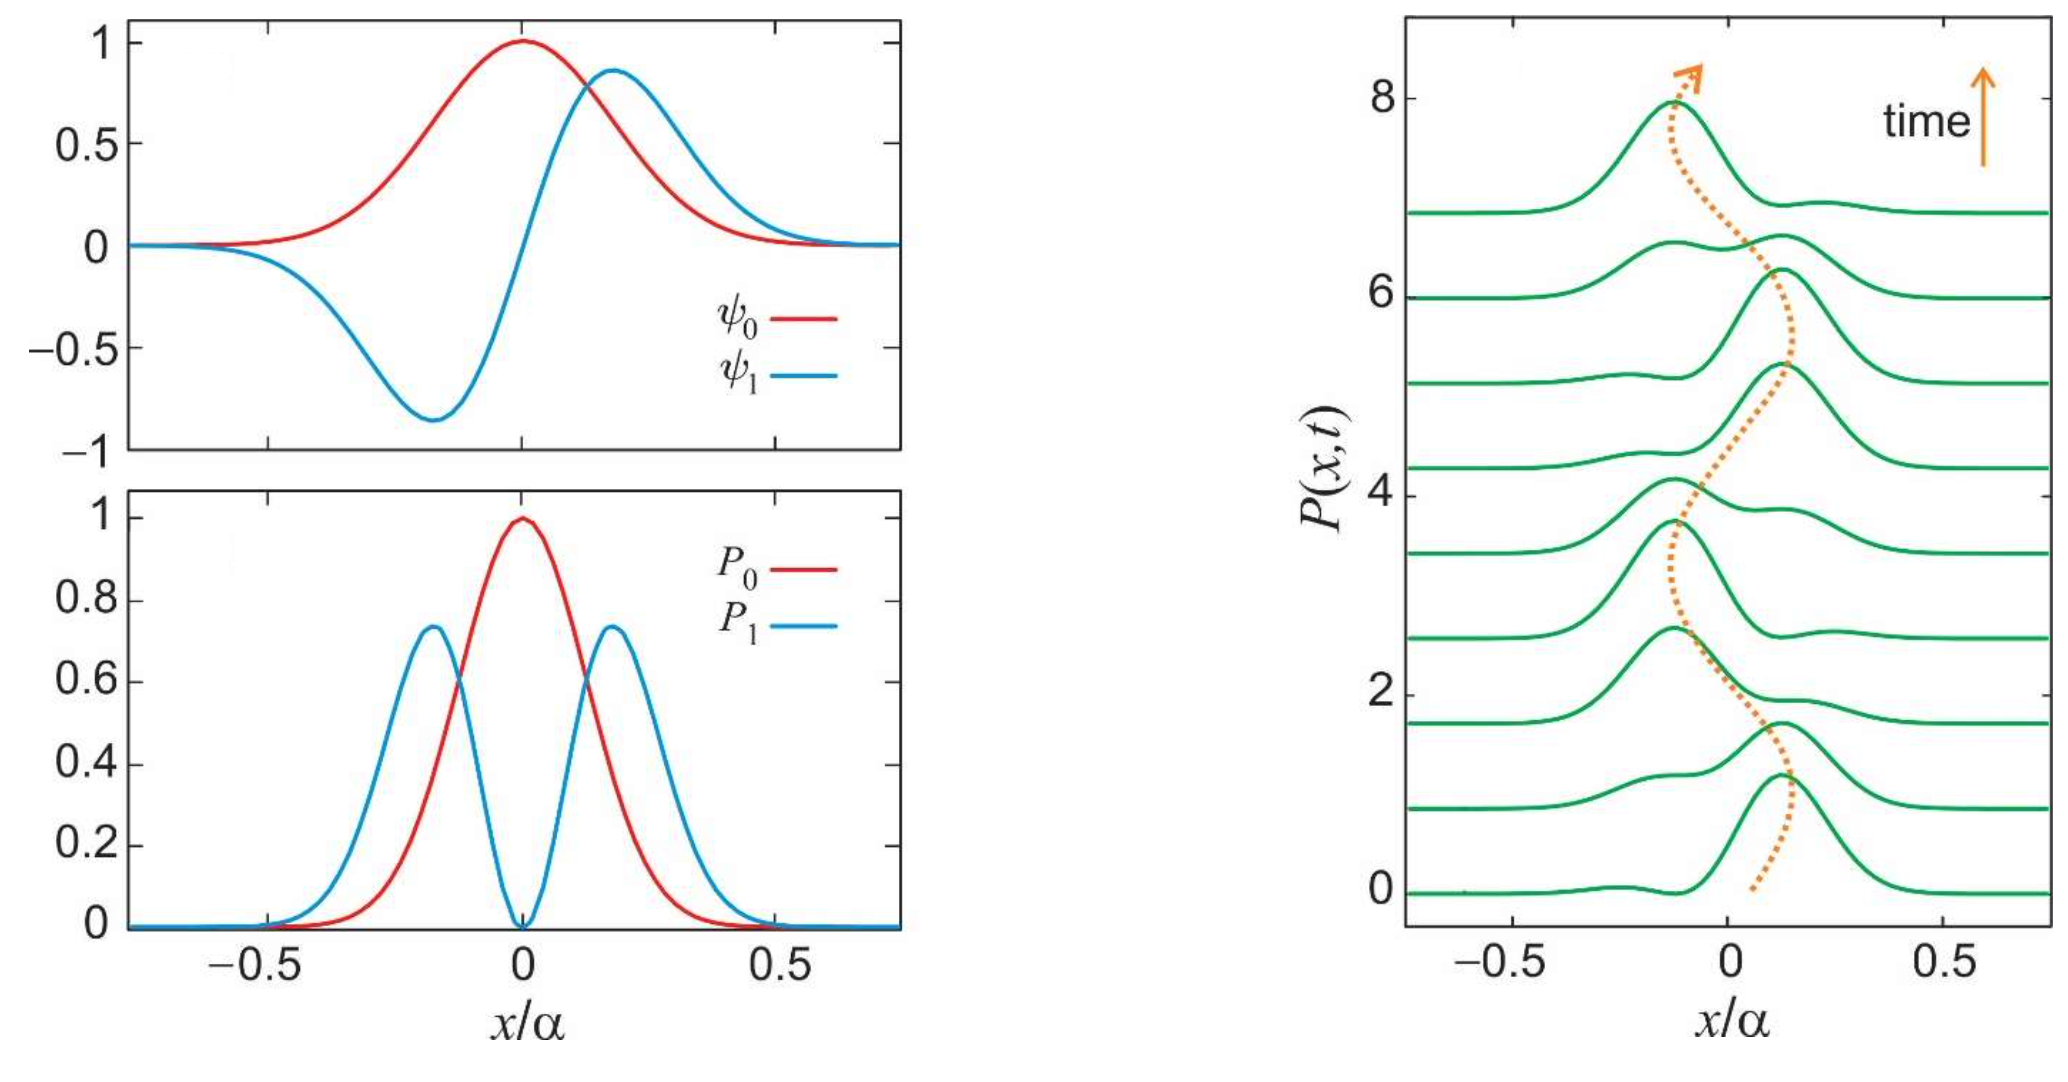
\includegraphics[width=0.7\linewidth]{lightCoupling.png}
        \caption{Light-induced coupling of quantum eigenstates.}
        \label{fig:lightCoupling}
    \end{figure}
    \begin{itemize}
        \item If we have two solutions to the particle in a box $\psi_0,\psi_1$ corresponding to the first and second energy levels, what light does is gives you a time-dependent wavefunction
        \begin{equation*}
            \psi(t) = c_0(t)\psi_0+c_1(t)\psi_1
        \end{equation*}
        \item The probability that the particle is in one state or the other oscillates: Since $c_n(t)=c_n\e[-iE_nt/\hbar]$,
        \begin{align*}
            P_1 &= |c_1(t)|^2 \approx \frac{\sin^2(E_1-E_0)t}{\hbar}&
            P_2 &= |c_0(t)|^2 \approx \frac{\cos^2(E_1-E_0)t}{\hbar}
        \end{align*}
    \end{itemize}
    \item Electronic degrees of freedom can be discussed in the same way.
    \begin{itemize}
        \item Light drives electrons back and forth (as per our classical molecule), but this time, we mathematically represent this change as a coupling of the $s$ orbital and the more elongated $p$ orbital.
    \end{itemize}
    \item Factors governing absorption strength.
    \begin{itemize}
        \item Beer's law.
        \item Two important factors.
        \begin{enumerate}
            \item Extinction coefficient.
            \item Concentration.
        \end{enumerate}
    \end{itemize}
    \item Quantum mechanically, absorption strength depends on state population.
    \begin{itemize}
        \item This is also a thermodynamic/statistical question.
        \item Thermal energy is distributed via the Boltzmann distribution.
        \item The probability of initially occupying an excited state increases with temperature.
    \end{itemize}
    \item Thermal energy distributes molecules through states with different rotational and vibrational states.
    \item Worry if $E_\text{rot}'',E_\text{vib}''\leq 2k_\text{B}T$.
    \item Populations at higher states will give rise to additional features in the absorption spectrum.
    \item Final states don't matter for us because $E_\text{final}\gg k_\text{B}T$.
    \begin{itemize}
        \item The only place where final energy matters is NMR because changes are so small; this is also why NMR is performed at cryogenic conditions.
    \end{itemize}
    \item Transition dipole moment.
    \begin{itemize}
        \item Classical (we need a change to grab onto) v. quantum (we take our transition dipole operator and square ite expected value) again.
    \end{itemize}
    \item Selection rules.
    \begin{itemize}
        \item Light can drive a molecule to go up or down one vibrational quantum. This is not strictly true because most oscillators are \emph{not} harmonic oscillators. Greater transitions are called \textbf{overtones}.
        \item Rotations: Same type of thing with $\Delta J=\pm 1$.
    \end{itemize}
\end{itemize}



\section{Office Hours (Moe)}
\begin{itemize}
    \item No Results and Discussion / short text summary/response section needed, right?
    \begin{itemize}
        \item Correct; none.
    \end{itemize}
    \item Do we need to calculate the extinction coefficient based on the Ocean Optics data?
    \begin{itemize}
        \item We don't.
    \end{itemize}
    \item What is the second table requested?
    \begin{itemize}
        \item Extend the reference data table.
    \end{itemize}
    \item Birge-Sponer plot for just $v'$ or both $v'$ and $v''$?
    \begin{itemize}
        \item Do present for the excited state.
        \item Create a grouped scatter plot for the ground state (5-6 data points for the value of 1, and the value of 2). Where there is overlap (i.e., everywhere we \emph{can} calculate $\Delta\omega(v'')$, we should).
    \end{itemize}
    \item Deriving the relationships between the Morse potential and the spectroscopic constants?
    \begin{itemize}
        \item You would have to do all of the stuff with the Laguerre polynomials and Schr\"{o}dinger equation.
    \end{itemize}
    \item Using the NIST database?
    \begin{itemize}
        \item Multiple database entries, look at the citations therein, and check the references in the manual.
        \item Worst case, contact them for values.
    \end{itemize}
    \item What is the value of the mercury calibration line? \SI{5461}{\angstrom}? My peak is at \SI{5483}{\angstrom}. Is this within the realm of possibility?
    \begin{itemize}
        \item Yes it is.
        \item We don't have to show this method now in the short lab report, but we would in the full lab report.
    \end{itemize}
    \item Help with Excel graph making: IodineHighRes plot.
    \begin{itemize}
        \item See practice plot.
    \end{itemize}
    \item Do we need to calculate errors?
    \begin{itemize}
        \item Yes, to the best of our ability based on what's in the manual.
    \end{itemize}
\end{itemize}



\section{Lecture 6: Infrared Vibrational-Rotational Spectroscopy}
\begin{itemize}
    \item \marginnote{1/19:}This is what's directly relevant to our \ce{HCl} experiment.
    \item Point of the online lectures: Provide more context on quantum dynamics, which are often glossed over.
    \item Review of the partitioning of quantum mechanical energies into electronic, vibrational, rotational, etc. DOFs.
    \begin{itemize}
        \item Different energy scales per DOF.
        \item We can treat electrons separately from nuclei using the BO approximation.
        \item Tokmakoff: "BO is the most important concept in molecular quantum mechanics."
        \item If we zoom into the bottom of the electronic potential well, we can see vibrational and rotational energy levels as per Figures \ref{fig:rotationQuantum}-\ref{fig:qmechEnergySpacing}.
        \begin{itemize}
            \item Note that this is only for one nuclear configuration! If we change the bond length, we have to redo the whole calculation.
        \end{itemize}
        \item We've been ignoring translational energy; if we want to understand how that influences our \ce{HCl} spectrum, come talk to Tokmakoff.
    \end{itemize}
    \item Up to this point, we've talked about how molecular parameters influence structure. Today, we do the opposite: Calculating said parameters from observables.
    \item Mid-IR light can induce vibrational and also rotational transitions.
    \item Typically, only one ground vibrational state is populated $v''=0$.
    \begin{itemize}
        \item Several rotational levels may be populated.
    \end{itemize}
    \item Simplest version of the spectrum.
    \begin{itemize}
        \item Heteronuclear diatomic molecule modeled as a quantum harmonic oscillator and rigid rotator.
        \item Under this approximation, we get equally spaced vibrational energy levels.
        \item First information from vibrational spectroscopy: Strength of bonding and shape of the potential well.
        \item Next, rotational energy: Gives bond length information.
    \end{itemize}
    \item Now for the light.
    \begin{itemize}
        \item Resonance condition: $h\nu=\Delta E$ again. Full formulas from the lab manuals written out.
    \end{itemize}
    \item Selection rules.
    \begin{itemize}
        \item $\Delta v=\pm 1$ and $\Delta J=\pm 1$.
        \item Differing transition frequency expressions for the R- and P-branches.
        \item If we're interested in the Q-branch, come talk to Tokmakoff.
    \end{itemize}
    \item $\nu_e$ is the spacing between the ground and first vibrational energy.
    \item R-branch and P-branch schematic.
    \begin{figure}[h!]
        \centering
        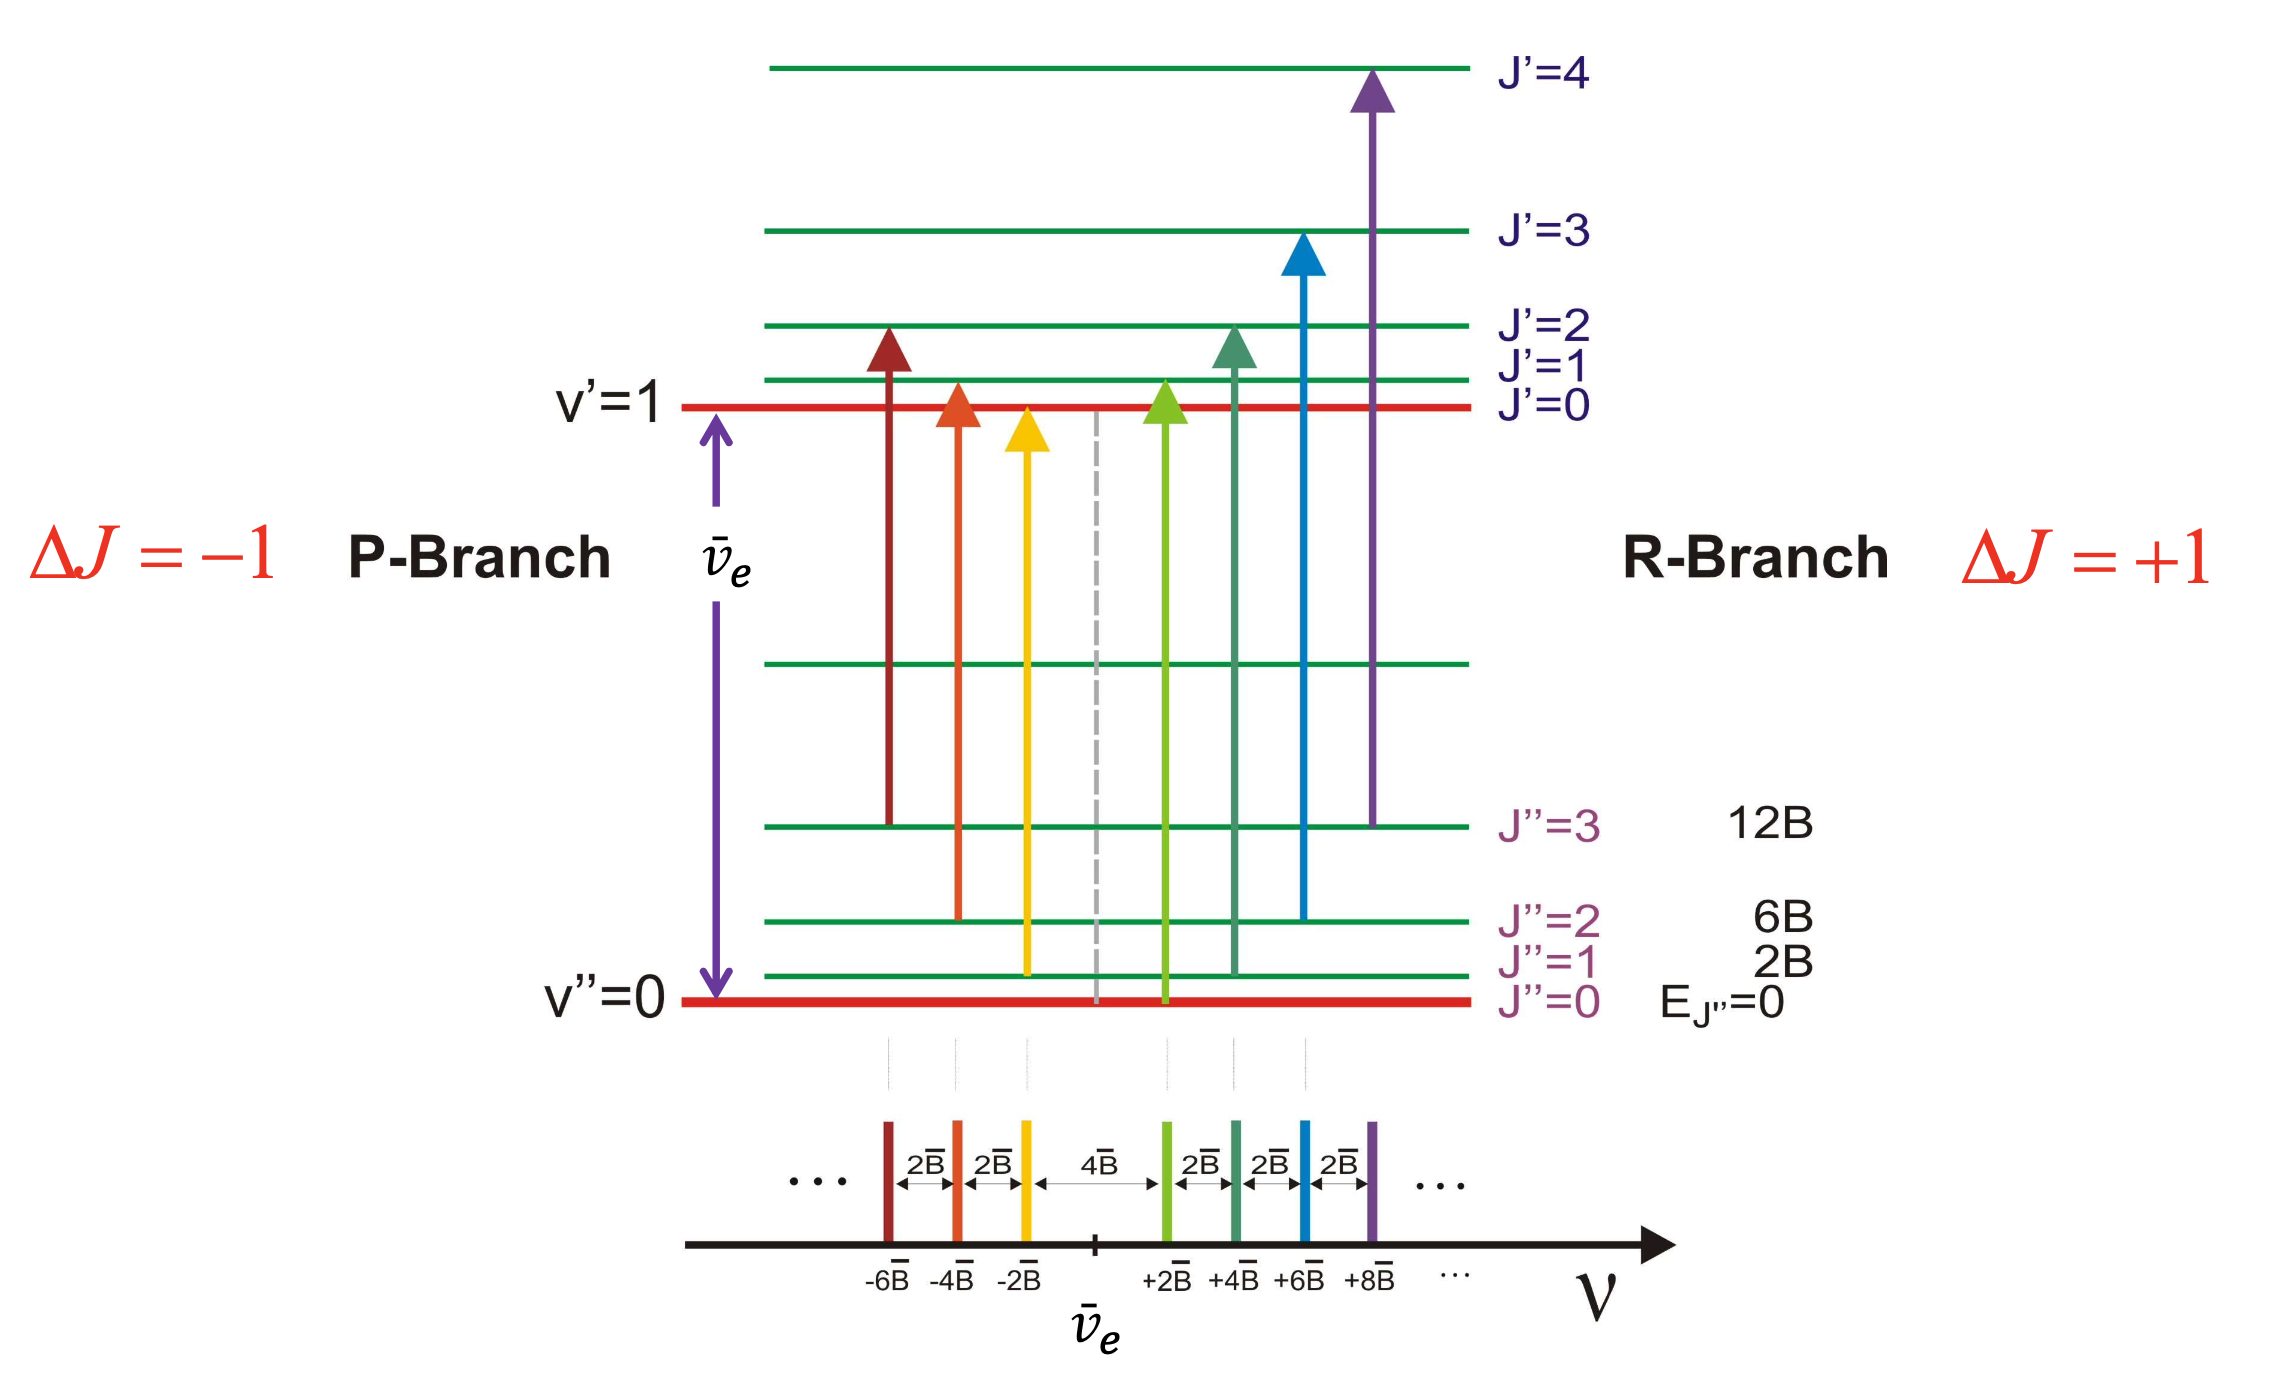
\includegraphics[width=0.7\linewidth]{roVibExcitations.png}
        \caption{Vibrational and rotational excitations.}
        \label{fig:roVibExcitations}
    \end{figure}
    \begin{itemize}
        \item Note the relationships between the selection rules and the transitions.
    \end{itemize}
    \item On a molecular level, we'd expect all lines to have the same intensity.
    \begin{itemize}
        \item In reality, occupation depends on temperature via the Boltzmann distribution.
        \item Great graphical explanation of the rotational energy levels!
    \end{itemize}
    \item Predicted vibrational-rotational spectrum.
    \begin{figure}[h!]
        \centering
        \begin{subfigure}[b]{0.6\linewidth}
            \centering
            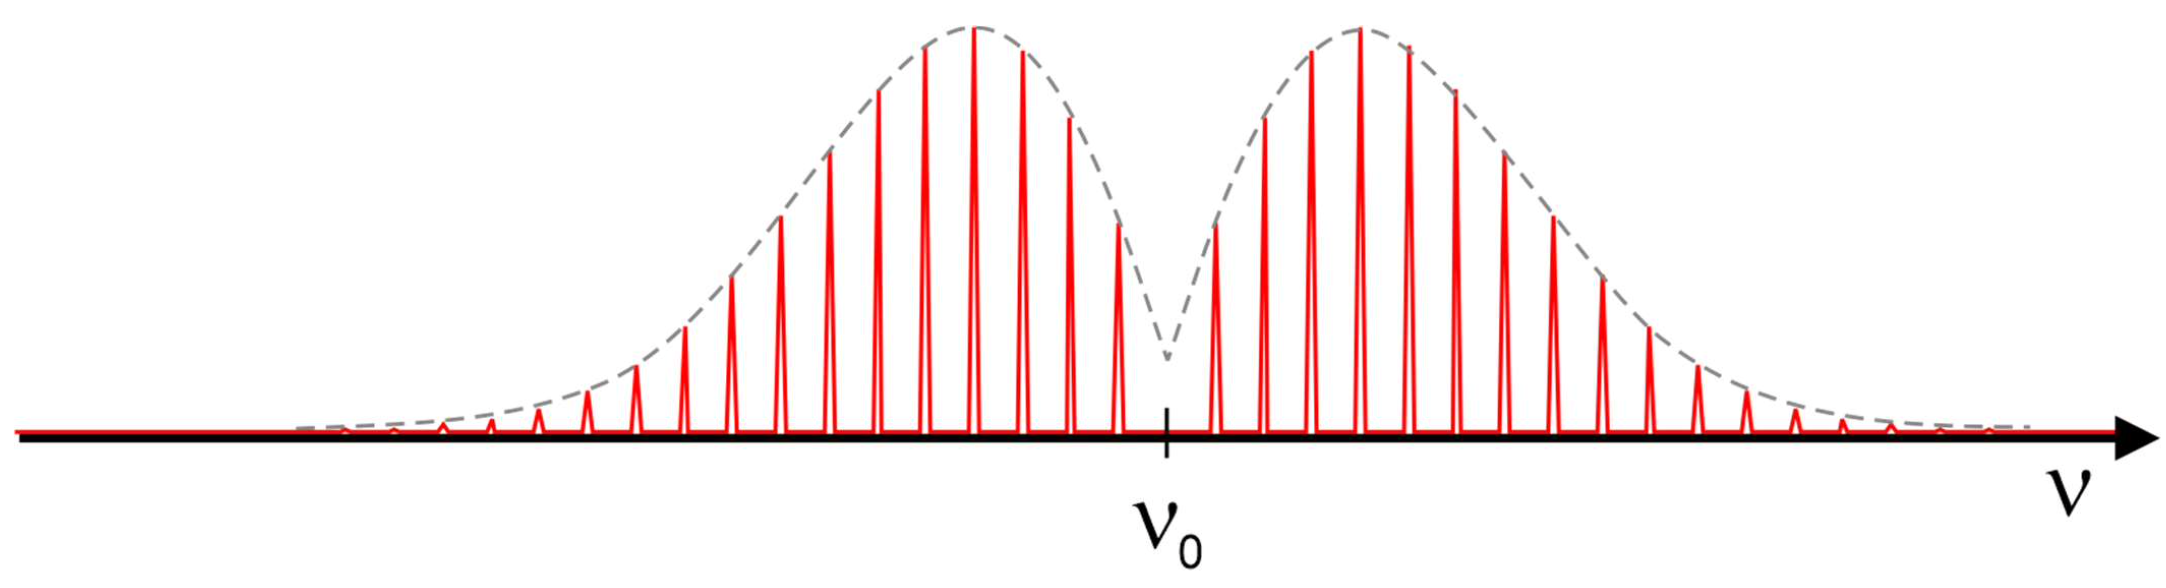
\includegraphics[width=0.8\linewidth]{PRdumbbella.png}
            \caption{Classical structure.}
            \label{fig:PRdumbbella}
        \end{subfigure}
        \begin{subfigure}[b]{0.6\linewidth}
            \centering
            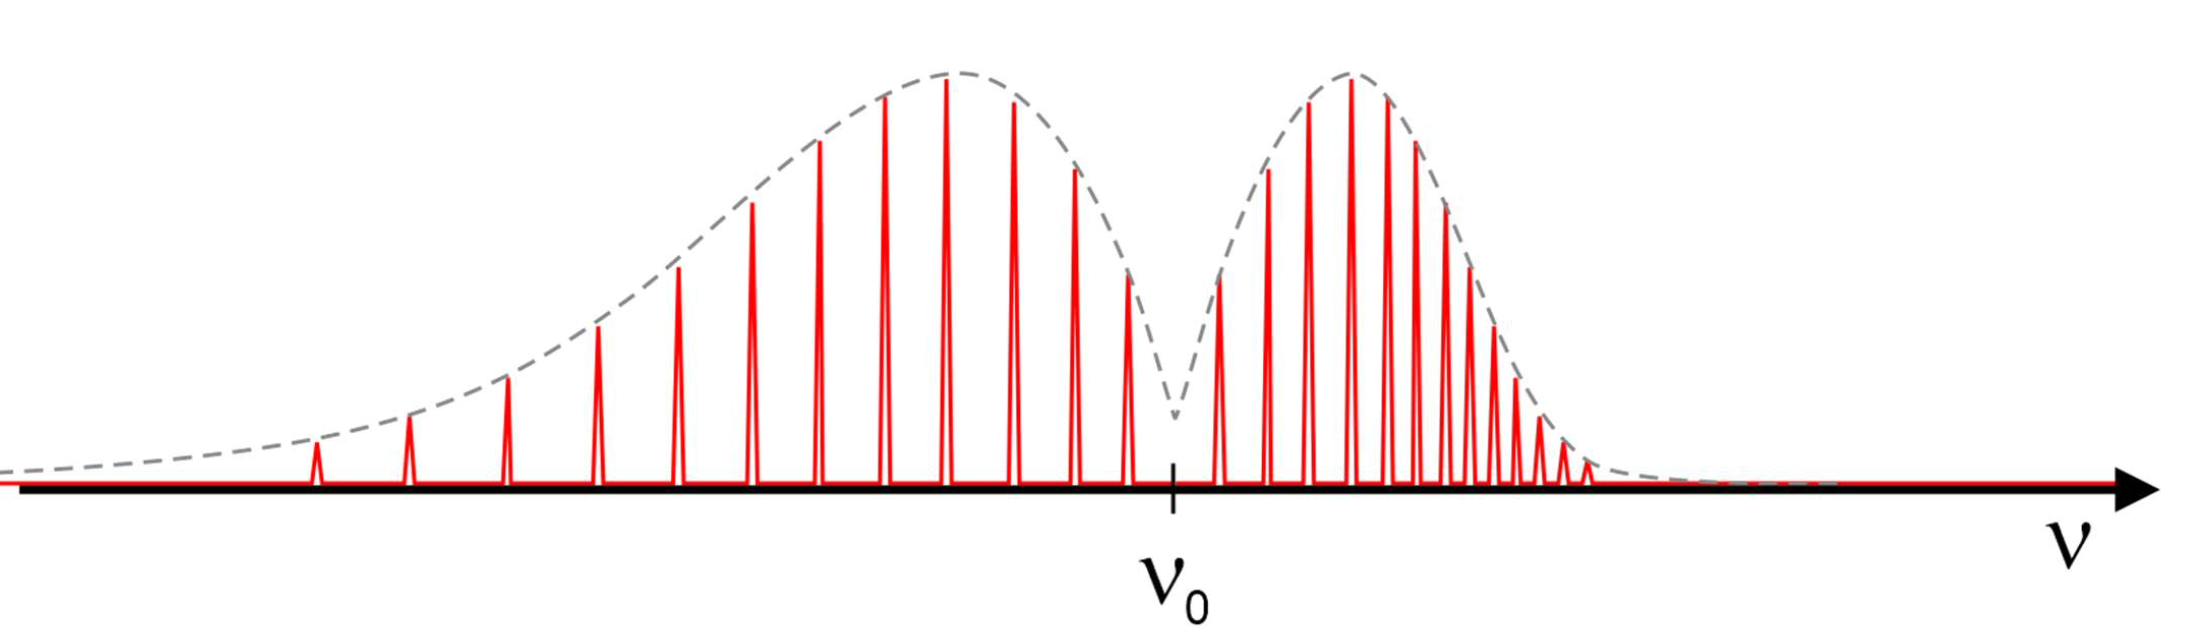
\includegraphics[width=0.8\linewidth]{PRdumbbellb.png}
            \caption{Real structure.}
            \label{fig:PRdumbbellb}
        \end{subfigure}
        \caption{Predicted and actual P/R-branch spacing.}
        \label{fig:PRdumbbell}
    \end{figure}
    \begin{itemize}
        \item See Figure \ref{fig:PRdumbbell}.
        \item The envelope gives you the classical structure (come talk to Tokmakoff about this).
        \item There are some other things to consider, e.g., Doppler shifts.
        \item In practice, our dumbbells shapes are not equally distributed. This problem is particularly bad for \ce{HCl}. Asymmetry induces this.
    \end{itemize}
    \item Vibration and rotation aren't independent.
    \begin{itemize}
        \item Vibration-rotation coupling --- if we resonantly excite a molecule, the bond length extends, the moment of inertial increases, and thus the molecules rotates more slowly.
        \item The equation
        \begin{equation*}
            \bar{B} = \bar{B}_e-\alpha_e\left( v+\frac{1}{2} \right)
        \end{equation*}
        is not theoretical; $\alpha_e$ is the experimentalist's fudge factor to get a more accurate moleucle.
        \item $\alpha_e$ is the vibrational-rotational coupling constant.
        \item Alternative: Centrifugal distortion. As the molecule spins faster, the bond length increases.
        \begin{equation*}
            \bar{B} = \bar{B}_e-D_eJ(J+1)
        \end{equation*}
        \item $D_e$ is the centrifugal distortion constant.
    \end{itemize}
    \item Vibrations aren't harmonic.
    \begin{itemize}
        \item Especially for strongly heteronuclear molecules such as \ce{HCl}.
        \item Atoms don't want to collide both because of the Coulombic repulsion between nuclei and the Pauli repulsion force between the electrons not wanting to occupy the same space.
        \item We account for the anharmonicity difference with another fudge factor.
        \item Overtone transitions.
    \end{itemize}
    \item Analysis of vibrational-rotational transition frequencies.
    \begin{itemize}
        \item We use a quadratic fit.
        \item The index parameter $m$ \emph{does} allow us to analyze both branches at the same time. Procedure:
        \begin{itemize}
            \item Assign transition frequencies to $J'',J',m$.
            \item Quadratic fit allows us to extract $\bar{v}_e,B_e,\alpha_e$.
            \item $B_e$ gives you $r_e$.
        \end{itemize}
    \end{itemize}
    \item Morse potential.
    \begin{itemize}
        \item It's hard to describe bonding with so few parameters, but the Morse potential does about as good a job as you can do. Additionally, there are analytical expressions relating our experimental parameters to $D_e,\beta$.
        \item Raise in your long report discussion how much you trust (or don't trust) the Morse potential.
        \begin{itemize}
            \item The potential gives you the dissociation energy $D_e$ of the molecule, but we're making measurements of vibrational energy levels at the very bottom of the well. What might that do?
            \item \ce{HCl} has a fairly long relaxation. More weakly bonded molecules have much steeper slopes (usually $\propto r^{-6}$).
        \end{itemize}
    \end{itemize}
    \item Next video: Polyatomic molecules, perhaps including \ce{CO2}.
    \item The bending vibration of \ce{CO2} has a Q-branch. Why? We should look into this.
    \item Another in-person lecture next Tuesday; same thing as today but for the \ce{I2} experiment.
\end{itemize}




\end{document}